\def\assignmenttitle{Energy consumption}
\def\assignmentdate{24-10-2011}
\def\coursetitle{02418 Statistical modelling}
\def\plotfolder{../plots}

\documentclass[11pt]{article}
\linespread{1}

\renewcommand{\thefootnote}{\fnsymbol{footnote}}

\usepackage{geometry} % see geometry.pdf on how to lay out the page. There's lots.
\usepackage[utf8]{inputenc}
\usepackage[T1]{fontenc}
\usepackage{array}
\usepackage{amsmath,amssymb,latexsym,epic,eepic,epsfig,graphics,psfrag}
\usepackage{amsfonts}
\usepackage{graphicx,float}
\usepackage{color}
\definecolor{mygray}{RGB}{244,244,244}
\definecolor{gray}{gray}{0.5}
\definecolor{myredish}{RGB}{193,33,97}
\definecolor{grayblue}{RGB}{91,112,142}
\definecolor{myorange}{RGB}{255,134,0}
\definecolor{green}{rgb}{0,0.4,0}

\usepackage[english]{babel}

\usepackage[bottom]{footmisc}

\usepackage{fancyhdr}
\pagestyle{fancy}
\lhead{\small\textit{Assignment \assignmentnumber -- 02417 Time Series Analysis -- Anders Hørsted (s082382)}}
\rhead{\thepage}
\chead{}
\lfoot{}\cfoot{}\rfoot{}

\usepackage{subfigure}
\usepackage{pstricks}
\usepackage{pst-node}
\usepackage{wrapfig}
\usepackage{caption}
\usepackage{multirow}
%\usepackage{fouriernc}
%\usepackage[charter]{mathdesign}
\usepackage{lmodern}
\usepackage[normalem]{ulem}
\geometry{a4paper} % or letter or a5paper or ... etc
% \geometry{landscape} % rotated page geometry

\usepackage{url}


\makeatletter
\renewcommand*\env@matrix[1][*\c@MaxMatrixCols c]{%
  \hskip -\arraycolsep
  \let\@ifnextchar\new@ifnextchar
  \array{#1}}
\makeatother

\newcommand\myimp{\quad\Leftrightarrow\quad}
\newcommand\half{\frac{1}{2}}
\newcommand\myvec[1]{\mathbf{#1}}
\newcommand\mymod[1]{\ (\text{mod }#1)}
\newcommand\myreal{\mathbb{R}}
\newcommand\mynatural{\mathbb{N}}
\newcommand\myinteger{\mathbb{Z}}
\newcommand\mycomplex{\mathbb{C}}
\newcommand\myint{\text{int}}
\newcommand\norm[1]{||\,#1\,||}
\newcommand\bignorm[1]{\big|\big|\,#1\,\big|\big|}
\newcommand\seq[1]{\big\{#1\big\}}
\newcommand\smallseq[1]{\{#1\}}
\newcommand\smallseqtoinf[1]{\smallseq{#1}_{k=1}^\infty}
\newcommand\lonew{\ell^1_w}
\newcommand\lone{\ell^1}
\newcommand\ltwo{\ell^2(\mynatural)}
\newcommand\ip[2]{\langle#1,#2\rangle}
\newcommand\hilbert[1]{\mathcal{#1}}
\newcommand\uinf{u_{\infty}}
\newcommand\erf{\text{erf\,}}
\newcommand\infint{\int_{\infty}^{\infty}}
\newcommand\fpi{FPI}
\newcommand\E[1]{\text{E}[#1]}
\newcommand\Var[1]{\text{Var}[#1]}
\newcommand\Cov[1]{\text{Cov}[#1]}
\newcommand\myverb[1]{{\footnotesize\texttt{#1}}}
\newcommand\Yhat{\widehat{Y}}
\newcommand\given{\,|\,}

\usepackage[scaled]{beramono}
\usepackage{listings}
\lstset {                 % A rudimentary config that shows off some features.
    language=R,
    basicstyle=\scriptsize\ttfamily, % Without beramono, we'd get cmtt, the teletype font.
    commentstyle=\textit, % cmtt doesn't do italics. It might do slanted text though.
    keywordstyle=,
    identifierstyle=,
    framextopmargin=4pt,
    framexbottommargin=4pt,
    framexleftmargin=4pt,
    framexrightmargin=4pt,
    xleftmargin=4pt,
    xrightmargin=4pt,
    backgroundcolor=\color{mygray},
    frame=single,
    showstringspaces=false,
    captionpos=b,
    tabsize=4            % Or whatever you use in your editor, I suppose.
}

\renewcommand{\lstlistlistingname}{Code Listings}
\renewcommand{\lstlistingname}{Code Listing}

\usepackage{tabulary}
\newcolumntype{y}{>{\centering\arraybackslash}R}

\title{\assignmenttitle}
\date{\assignmentdate}
\author{Assignment \assignmentnumber\ -- 02417 Time Series Analysis -- Anders Hørsted (s082382)}
%\author{}
\date{} % delete this line to display the current date



\begin{document}

\maketitle

In this case models for the heat consumption of houses are build. The models are fitted to a data set containing measurements of heat consumption along with 4 other environmental variables as well as the date of the measurement for 16 different houses. First a model is build that only uses data for a single house. Then this model is extended to try to make a general model that includes all 16 houses.

\section*{Model for one house}
First a model for a single house is developed. The model will be based on the house with \myverb{id=5} and as a first step a plot of the heat consumption as function of the date is plotted in figure~\ref{fig:Q-house-5}. As seen the heat consumption $Q$ depends primary on the season with large $Q$ in the winter and small $Q$ in the summer. \par
For the heat loss across a wall we have that 
\begin{equation*}
    Q_w = U_a(T_a - T_i)
\end{equation*}
where $T_a$ is the ambient temperature, $T_i$ the indoor temperature and $U_a$ is the response from temperature differences. We regard $T_i$ as a constant and therefore get the simple relationship $Q_w = U_aT_a + k$. If heat loss across the wall was the only way that energy could flow in/out of the house, a great fit for the data should be obtained by the linear model \myverb{Q\texttildelow Ta}.
\begin{figure}[ht]
\centering
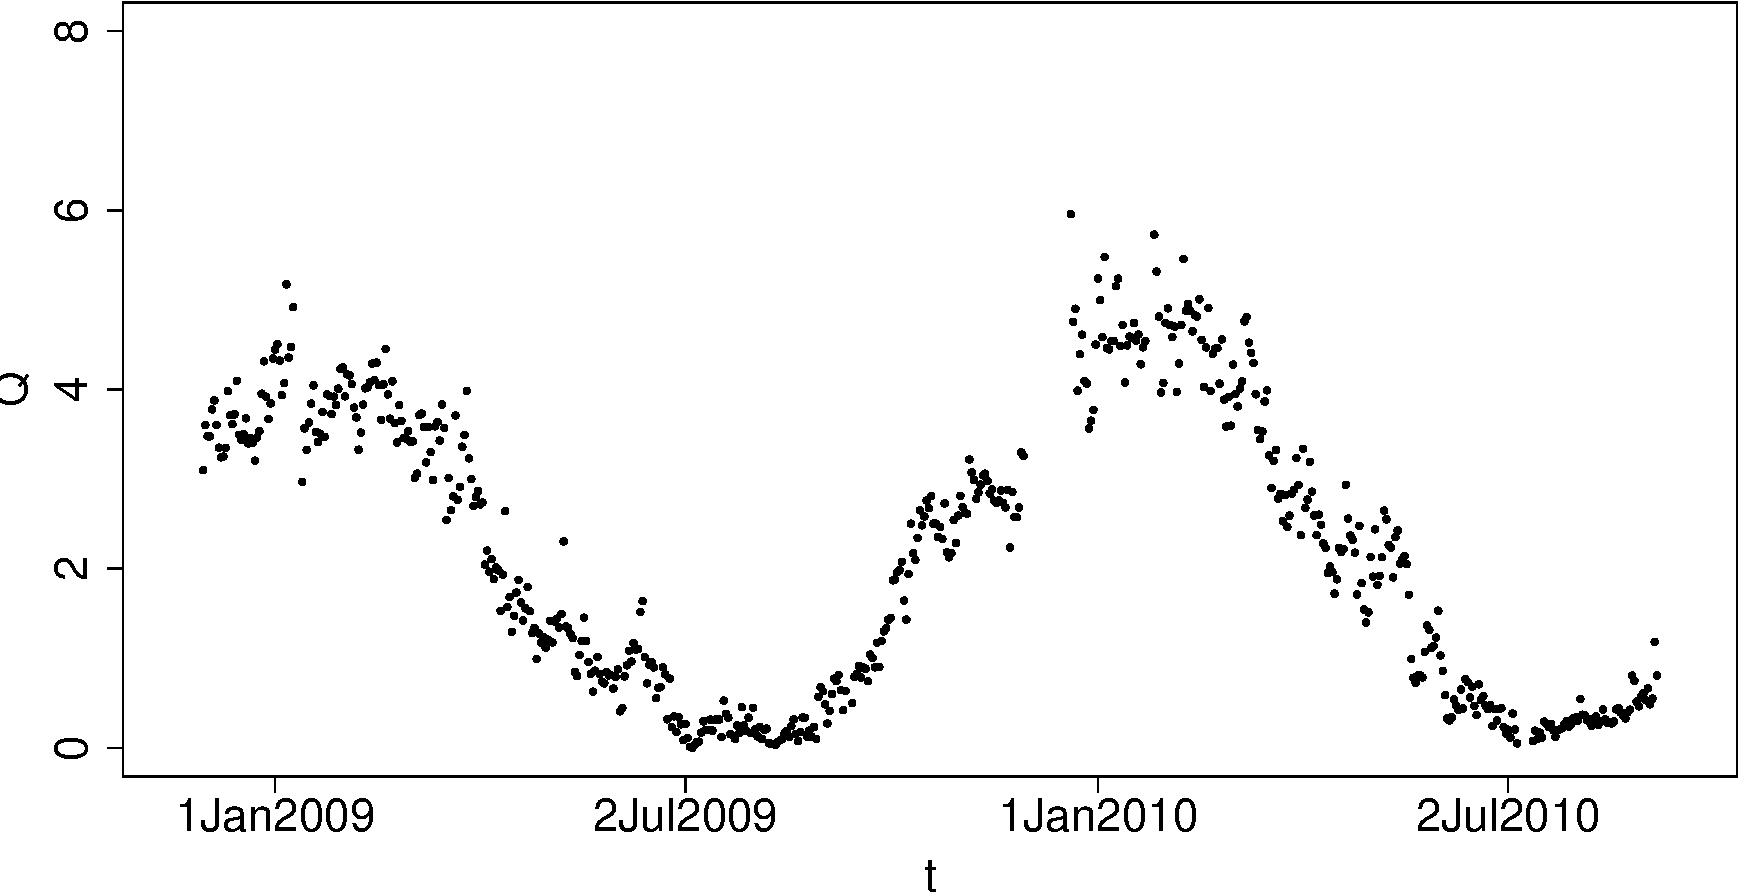
\includegraphics[width=110mm]{\plotfolder/Q-h05.pdf}
\caption{Heat consumption for house 5.}
\label{fig:Q-house-5}
\end{figure}

\subsection*{Fitting the simple model for one house}
\begin{table}[ht]
    \centering
    % latex table generated in R 2.10.1 by xtable 1.5-6 package
% Tue Oct 25 17:25:13 2011
\begin{tabular}{rrrrr}
  \hline
 & Estimate & Std. Error & t value & Pr($>$$|$t$|$) \\ 
  \hline
(Intercept) & 3.9542 & 0.0270 & 146.56 & 0.0000 \\ 
  Ta & -0.2123 & 0.0024 & -87.41 & 0.0000 \\ 
   \hline
\end{tabular}

    \caption{Summary table for the simple model for house 5}\label{tbl:onehouse-m1}
\end{table}
Fitting the simple model \myverb{Q\texttildelow Ta} in R gives the output shown in table~\ref{tbl:onehouse-m1} and the diagnostic plots in figure~\ref{fig:onehouse-m1-diagnostics}. From the plots the residuals are seen to be approximately normal distributed, but the variance do not seem to be independent of the fitted values. The primary problem is that our model makes negative predictions which doesn't make sense since $Q$ is the energy consumption of the house. This is also seen by the fact that the residuals for negative fitted values lies on an approximately straigth line with a slope of -1. Therefore all values that are predicted as negative have an observed value close to 0. More problematic is it that the residuals for fitted values in the interval $(0,2)$ seems to have a negative mean and variance smaller than for fitted values larger than 2. To get a idea of how the model can be extended the residuals are plotted against the predictors. The most interesting predictor turn out to be $T_a$ and this plot is shown in figure~\ref{fig:onehouse-m1-expla-res}. 
\begin{figure}[ht]
    \centering
    \mbox{\subfigure{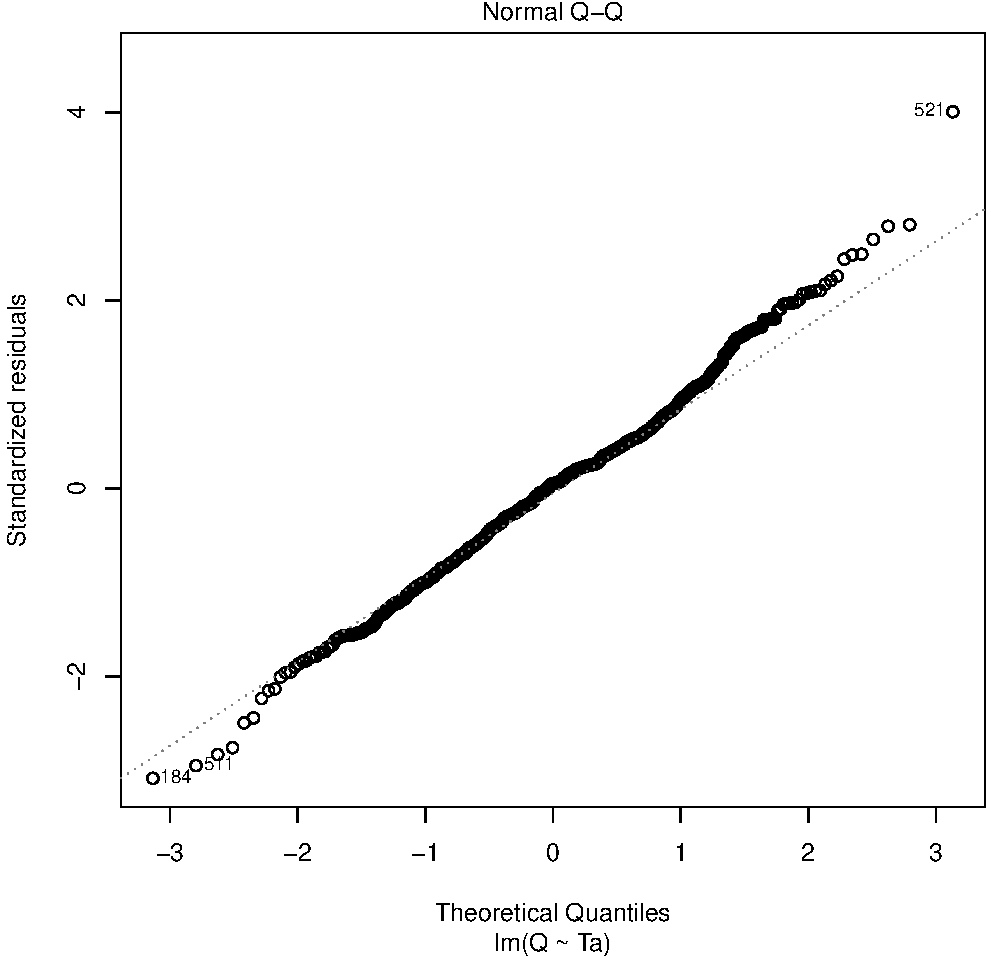
\includegraphics[width=70mm]{../plots/one-house-m1-qq-plot.pdf}} \quad 
          \subfigure{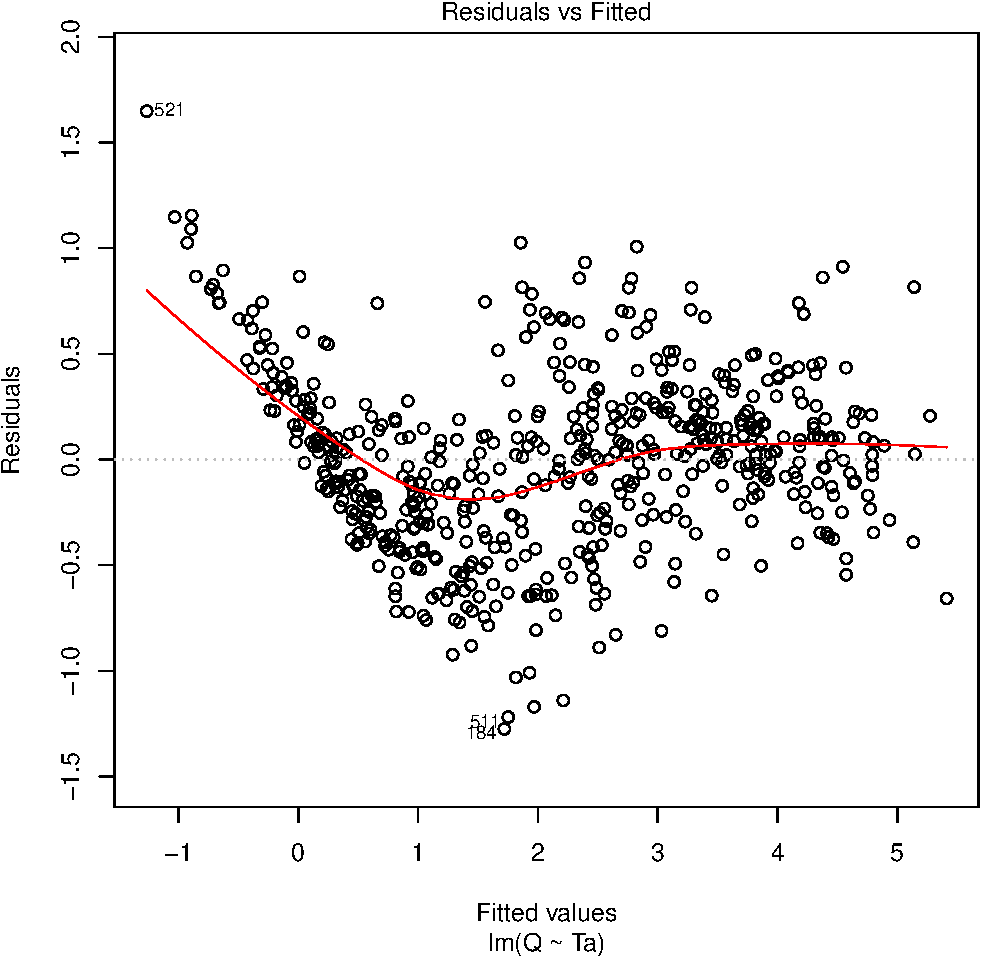
\includegraphics[width=70mm]{../plots/one-house-m1-fit-res-plot.pdf}}}
    \caption{Diagnostic plots for simple model for house 5}
    \label{fig:onehouse-m1-diagnostics}
\end{figure}
\begin{figure}[ht]
    \centering
    \mbox{\subfigure{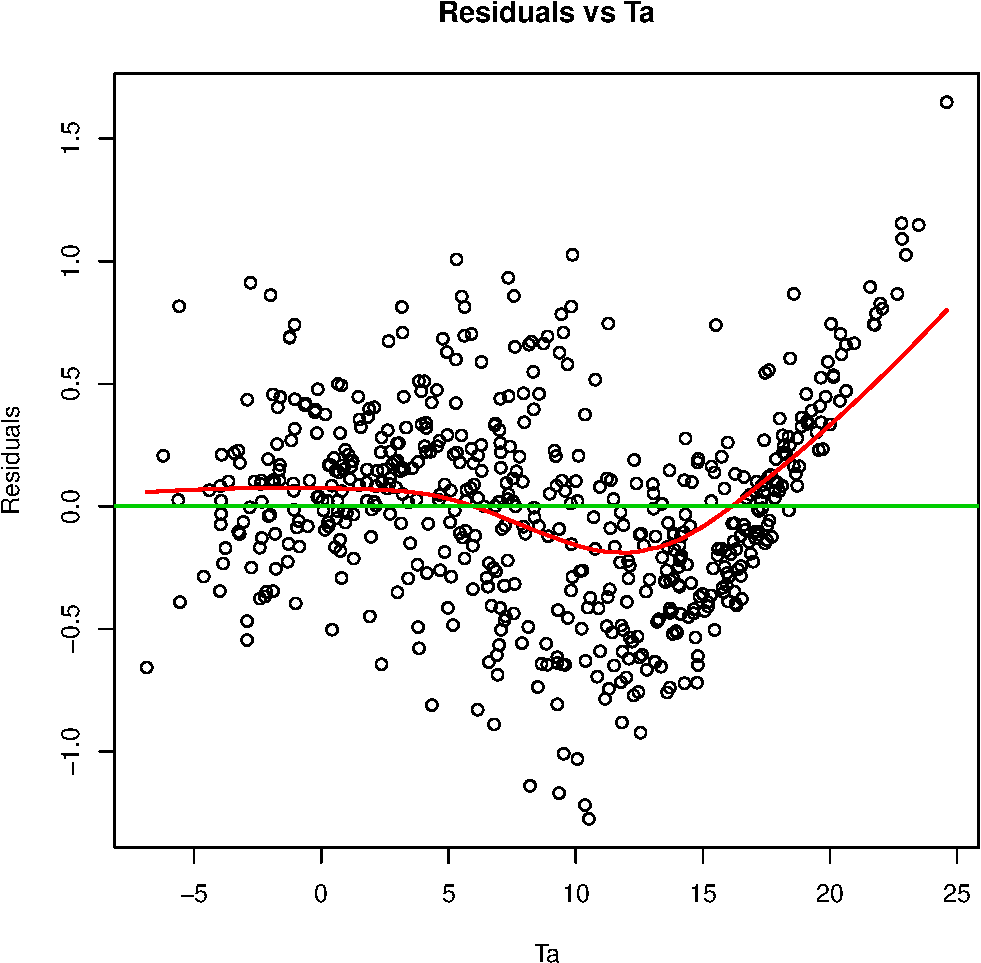
\includegraphics[width=70mm]{../plots/one-house-m1-Ta-data-plot.pdf}}}
    \caption{Residuals vs $T_a$ for simple model for house 5}
    \label{fig:onehouse-m1-expla-res}
\end{figure}
\subsection*{Fitting a higher order polynomial in $T_a$}
From the plot of the residuals vs $T_a$ it is seen that for high values of $T_a$ the residuals are consistently above 0. A way to counteract this is by fitting a higher order polynomial in $T_a$. After testing a few different degrees a 3 degree polynomial seems to be of the right complexity. The model is defined as \myverb{Q\texttildelow poly(Ta, 3, raw=TRUE))} which gives the coefficients in table~\ref{tbl:onehouse-m2} and the diagnostic plots in figure~\ref{fig:onehouse-m2-diagnostics}. It is seen that the residuals vs fitted values shows much less structure now which is as wished. Also the model no longer predicts negative values of $Q$ which is great. On the other hand the residuals begins to be s-shaped in the QQ-plot which indicates a distribution with 'fat tails' compared to the normal distribution. The conclusion is that the 3 degree polynomial model do seem to fit the data well but the deviation from normallity shown in the QQ plot is unsatisfying. The next step is to use information from the other predictors.

\begin{table}[ht]
    \centering
    % latex table generated in R 2.10.1 by xtable 1.5-6 package
% Tue Oct 25 18:02:07 2011
\begin{tabular}{rrrrr}
  \hline
 & Estimate & Std. Error & t value & Pr($>$$|$t$|$) \\ 
  \hline
(Intercept) & 4.1276 & 0.0245 & 168.41 & 0.0000 \\ 
  poly(Ta, 3, raw = TRUE)1 & -0.2035 & 0.0069 & -29.53 & 0.0000 \\ 
  poly(Ta, 3, raw = TRUE)2 & -0.0094 & 0.0010 & -9.55 & 0.0000 \\ 
  poly(Ta, 3, raw = TRUE)3 & 0.0005 & 0.0000 & 13.08 & 0.0000 \\ 
   \hline
\end{tabular}

    \caption{Summary table for the third degree polynomial model for house 5}\label{tbl:onehouse-m2}
\end{table}
\begin{figure}[ht]
    \centering
    \mbox{\subfigure{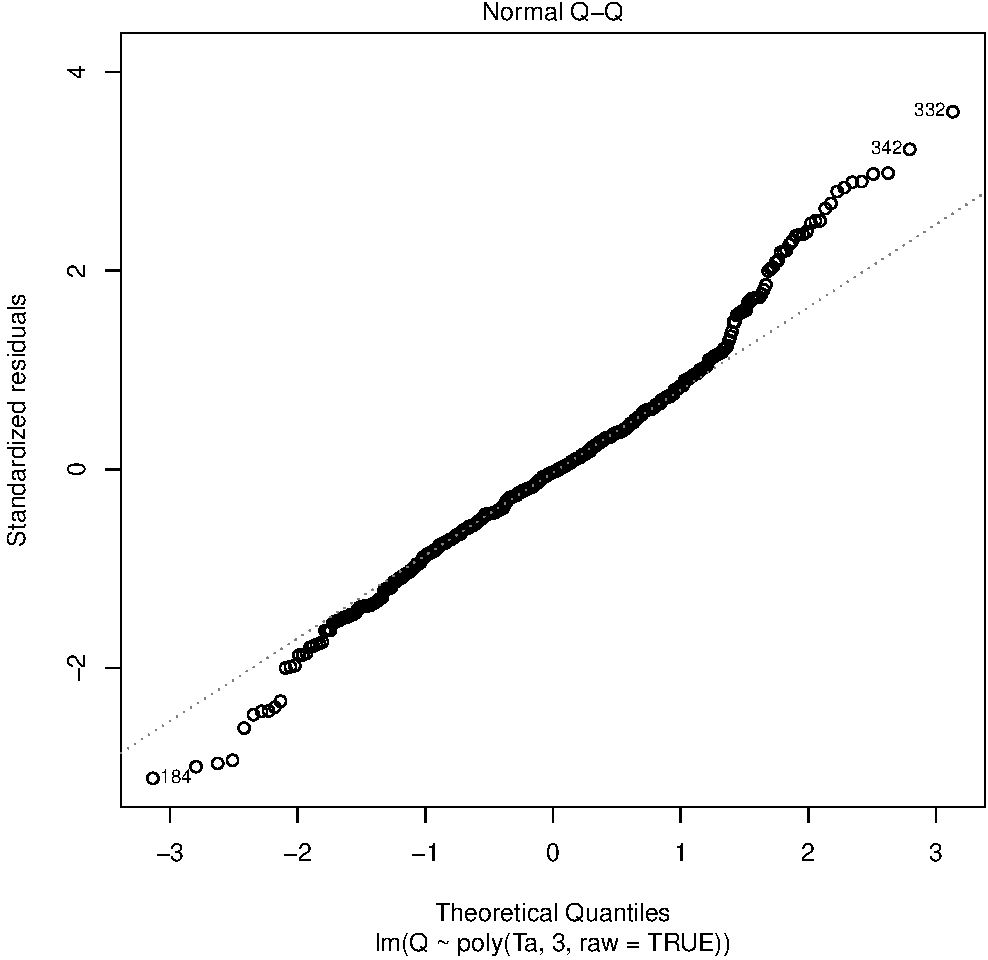
\includegraphics[width=70mm]{../plots/one-house-m2-qq-plot.pdf}} \quad 
          \subfigure{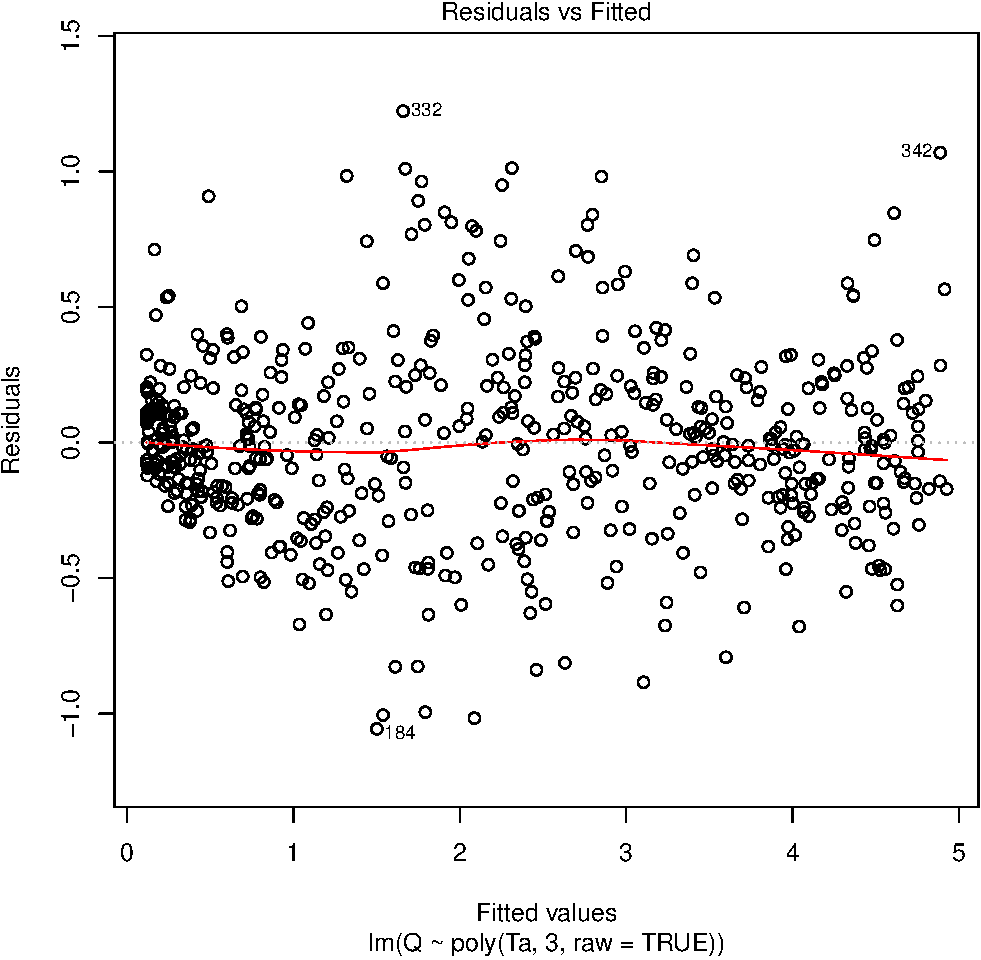
\includegraphics[width=70mm]{../plots/one-house-m2-fit-res-plot.pdf}}}
    \caption{Diagnostic plots for the third degree polynomial model for house 5}
    \label{fig:onehouse-m2-diagnostics}
\end{figure}

\subsection*{Adding predictors to the 3 degree polynomial model}
\begin{table}[ht]
    \centering
    % latex table generated in R 2.10.1 by xtable 1.5-6 package
% Tue Oct 25 18:36:56 2011
\begin{tabular}{rrrrr}
  \hline
 & Estimate & Std. Error & t value & Pr($>$$|$t$|$) \\ 
  \hline
(Intercept) & 4.4334 & 0.0525 & 84.46 & 0.0000 \\ 
  poly(Ta, 3, raw = TRUE)1 & -0.1779 & 0.0067 & -26.49 & 0.0000 \\ 
  poly(Ta, 3, raw = TRUE)2 & -0.0070 & 0.0009 & -7.75 & 0.0000 \\ 
  poly(Ta, 3, raw = TRUE)3 & 0.0004 & 0.0000 & 10.94 & 0.0000 \\ 
  Ws & 0.0129 & 0.0118 & 1.09 & 0.2779 \\ 
  G & -0.0006 & 0.0002 & -2.63 & 0.0088 \\ 
  sunElev & -1.4168 & 0.1933 & -7.33 & 0.0000 \\ 
   \hline
\end{tabular}

    \caption{Summary table for the model in (\ref{eq:m3})}\label{tbl:onehouse-m3}
\end{table}
Now the model given as
\begin{equation}\label{eq:m3}
    Q = \beta_1T_a + \beta_2T_a^2 + \beta_3T_a^3 + \beta_4W_s + \beta_5G + \beta_6S_{elev} + \beta_7 + \varepsilon
\end{equation}
is fitted to the data. The coefficients are shown in table~\ref{tbl:onehouse-m3} and it is seen that some of the predictors might be redundant. To trim the model a stepwise selection is performed. The result is that $W_s$ is dropped from the model. The model is then given as
\begin{equation}\label{eq:m4}
    Q = \beta_1T_a + \beta_2T_a^2 + \beta_3T_a^3 +  \beta_4G + \beta_5S_{elev} + \beta_6 + \varepsilon
\end{equation}
When this model is fitted to the data the coefficients in table~\ref{tbl:onehouse-m4} are obtained. The diagnostic plots are shown in figure~\ref{fig:onehouse-m4-diagnostics}. From the QQ plot it seems as if the residuals are slightly closer to a normal distribution but it isn't very significant compared to the model with only a third degree polynomial in $T_a$. For now the predictors are kept in the model though and the next step is to look for possible interaction terms to include.
\begin{table}[ht]
    \centering
    % latex table generated in R 2.10.1 by xtable 1.5-6 package
% Tue Oct 25 18:49:01 2011
\begin{tabular}{rrrrr}
  \hline
 & Estimate & Std. Error & t value & Pr($>$$|$t$|$) \\ 
  \hline
(Intercept) & 4.4671 & 0.0424 & 105.47 & 0.0000 \\ 
  poly(Ta, 3, raw = TRUE)1 & -0.1763 & 0.0066 & -26.91 & 0.0000 \\ 
  poly(Ta, 3, raw = TRUE)2 & -0.0072 & 0.0009 & -8.05 & 0.0000 \\ 
  poly(Ta, 3, raw = TRUE)3 & 0.0004 & 0.0000 & 11.09 & 0.0000 \\ 
  G & -0.0006 & 0.0002 & -2.62 & 0.0091 \\ 
  sunElev & -1.4239 & 0.1932 & -7.37 & 0.0000 \\ 
   \hline
\end{tabular}

    \caption{Summary table for the model in (\ref{eq:m4})}\label{tbl:onehouse-m4}
\end{table}
\begin{figure}[ht]
    \centering
    \mbox{\subfigure{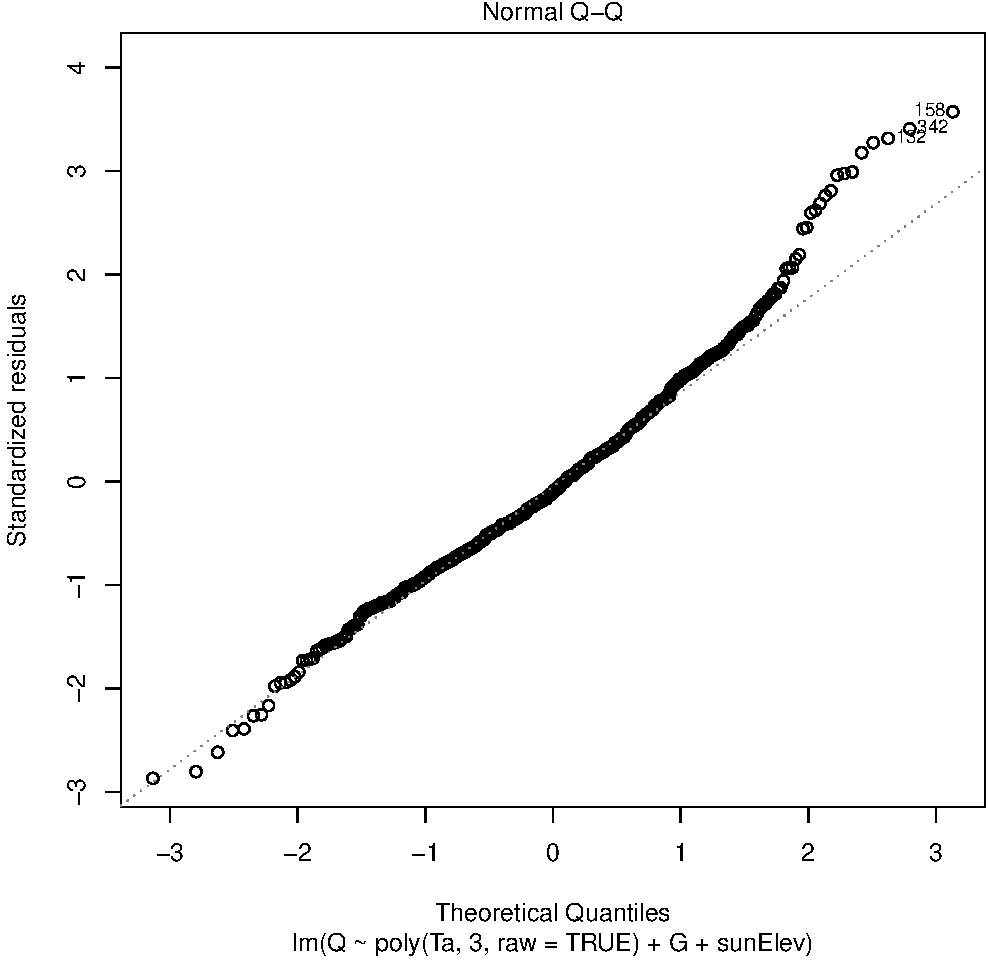
\includegraphics[width=70mm]{../plots/one-house-m4-qq-plot.pdf}} \quad 
          \subfigure{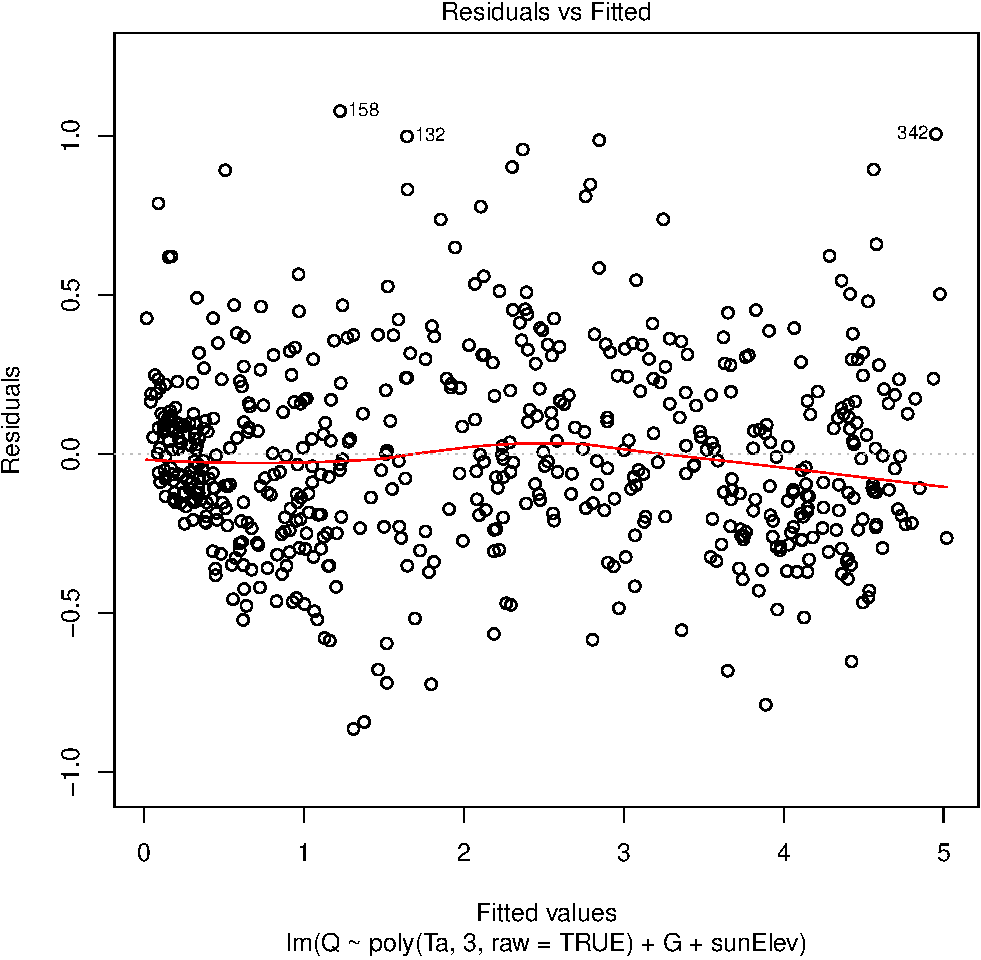
\includegraphics[width=70mm]{../plots/one-house-m4-fit-res-plot.pdf}}}
    \caption{Diagnostic plots for the model in (\ref{eq:m4})}
    \label{fig:onehouse-m4-diagnostics}
\end{figure}

\subsection*{Including interaction terms}
There are 4 predictor variables which gives 6 unique interaction pairs to test. One idea is to include all pairs in a model and then do a stepwise selection to get rid of redundant pairs. First a single interaction pair is tested though. The interaction between the ambient temperature and the wind speed might be interesting since low temperature combined with high wind speed could mean increased flow of cold air through windows. The model given by
\begin{equation}\label{eq:m5}
    Q = \beta_1T_a + \beta_2T_a^2 + \beta_3T_a^3 +  \beta_4G + \beta_5S_{elev} + \beta_6W_s + \beta_7T_aW_s + \beta_8 + \varepsilon
\end{equation}

\textit{Due to bad time management this is unfortunately how far I get before hand-in. The summary table and diagnostics plots for the model with interaction are shown in table~\ref{tbl:onehouse-m5} and figure~\ref{fig:onehouse-m5-diagnostics}.}

\begin{table}[ht]
    \centering
    % latex table generated in R 2.10.1 by xtable 1.5-6 package
% Tue Oct 25 19:35:53 2011
\begin{tabular}{rrrrr}
  \hline
 & Estimate & Std. Error & t value & Pr($>$$|$t$|$) \\ 
  \hline
(Intercept) & 4.3764 & 0.0594 & 73.71 & 0.0000 \\ 
  poly(Ta, 3, raw = TRUE)1 & -0.1710 & 0.0075 & -22.78 & 0.0000 \\ 
  poly(Ta, 3, raw = TRUE)2 & -0.0068 & 0.0009 & -7.41 & 0.0000 \\ 
  poly(Ta, 3, raw = TRUE)3 & 0.0004 & 0.0000 & 10.51 & 0.0000 \\ 
  Ws & 0.0378 & 0.0170 & 2.22 & 0.0268 \\ 
  G & -0.0006 & 0.0002 & -2.58 & 0.0102 \\ 
  sunElev & -1.4215 & 0.1927 & -7.37 & 0.0000 \\ 
  Ws:Ta & -0.0037 & 0.0018 & -2.03 & 0.0424 \\ 
   \hline
\end{tabular}

    \caption{Summary table for the model in (\ref{eq:m5})}\label{tbl:onehouse-m5}
\end{table}
\begin{figure}[ht]
    \centering
    \mbox{\subfigure{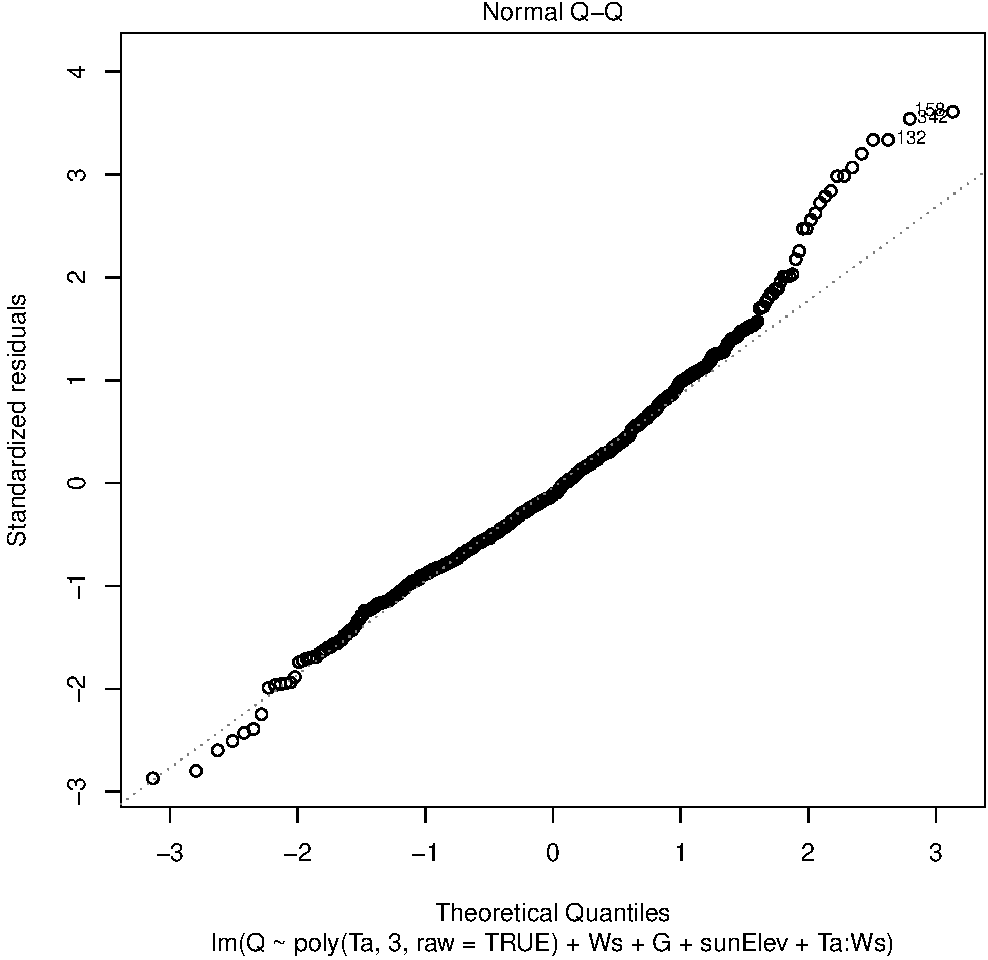
\includegraphics[width=70mm]{../plots/one-house-m5-qq-plot.pdf}} \quad 
          \subfigure{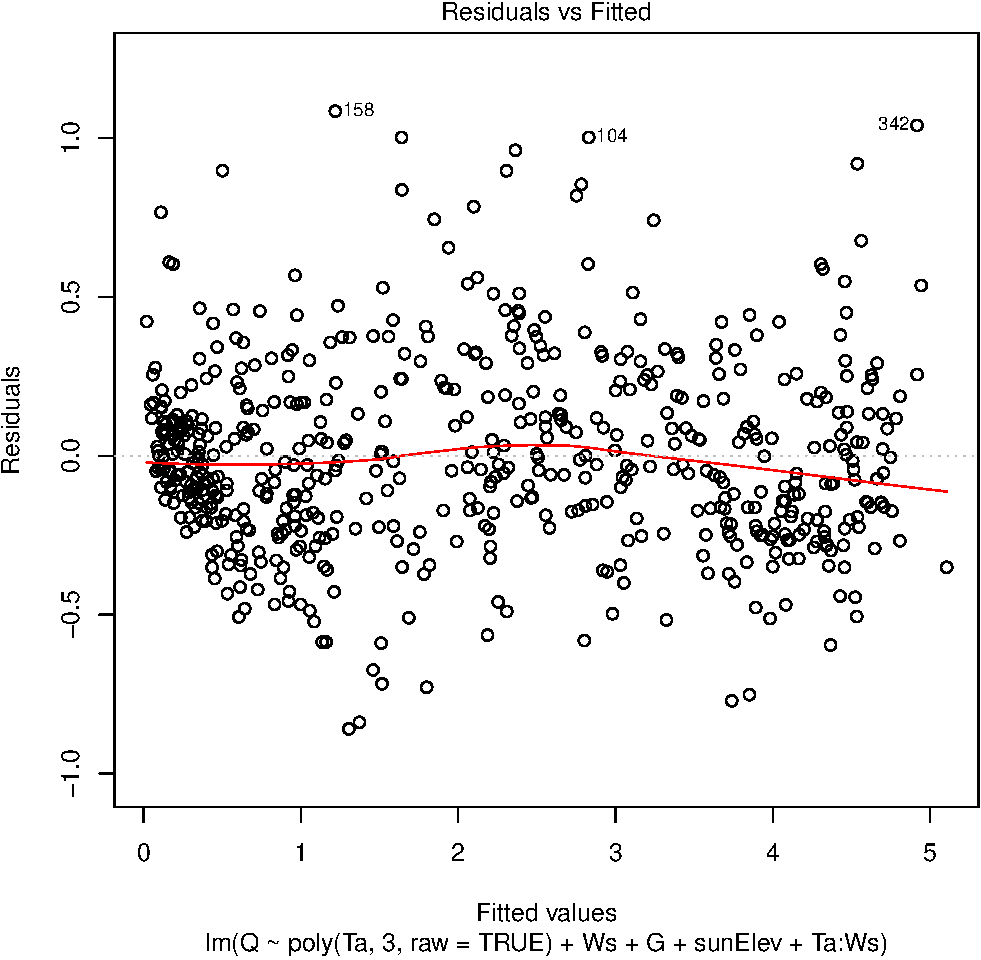
\includegraphics[width=70mm]{../plots/one-house-m5-fit-res-plot.pdf}}}
    \caption{Diagnostic plots for the model in (\ref{eq:m5})}
    \label{fig:onehouse-m5-diagnostics}
\end{figure}

\pagebreak

\renewcommand\thesection{\Alph{section}}
\section{Appendices}
All R source code is included in the appendices. All the source code including the Latex code used for the report can also be found at \url{https://github.com/alphabits/dtu-fall-2011/tree/master/02418/heat-consumption}.
\subsection{functions.R}
\lstinputlisting{../src/functions.R}
\subsection{loaddata.R}
\lstinputlisting{../src/loaddata.R}
\subsection{eda.R}
\lstinputlisting{../src/eda.R}
\subsection{singlehouse.R}
\lstinputlisting{../src/singlehouse.R}

\pagebreak
\begin{thebibliography}{9}

\bibitem{hm}
  Henrik Madsen,
  \emph{Time Series Analysis}.
  Chapman \& Hall/CRC,
  1st Edition,
  2008.

%\bibitem{taleb}
%  Nassim Nicholas Taleb,
%  \emph{The Black Swan}.
%  Random House Trade Paperbacks
%  2nd Edition,
%  2010.

\end{thebibliography}


\end{document}
